% Cal Poly Thesis
% 
% based on UC Thesis format
%
% modified by Mark Barry 2/07.
%
%presented by Scott Winkleblack
%

\documentclass[12pt]{ucthesis}
\usepackage{ifpdf}

\newif\ifpdf
\ifx\pdfoutput\undefined
    \pdffalse % we are not running PDFLaTeX
\else
\pdfoutput=1 % we are running PDFLaTeX
\pdftrue \fi

\usepackage{url}
\usepackage{multicol}
\usepackage{cite}

\usepackage{fixltx2e}

\usepackage{tabu}

\usepackage [english]{babel}
\usepackage [autostyle, english = american]{csquotes}
\MakeOuterQuote{"}

\usepackage{listings}

\ifpdf
    \usepackage[pdftex]{graphicx}
    % Update title and author below...
    \usepackage[pdftex,plainpages=false,breaklinks=true,colorlinks=true,urlcolor=blue,citecolor=blue,
		linkcolor=blue,bookmarks=true,bookmarksopen=true,%
		bookmarksopenlevel=3,pdfstartview=FitV,
		pdfauthor={Connor Citron},
		pdftitle={Stereo Vision System Module for Low-Cost FPGAs for Autonomous Mobile Robots},
		pdfkeywords={thesis, masters, cal poly}]{hyperref}
    %Options with pdfstartview are FitV, FitB and FitH
    \pdfcompresslevel=1

\else
    \usepackage{graphicx}
\fi

\usepackage{hyperref}
\hypersetup{
	linktoc=all,
    colorlinks,
    citecolor=black,
    filecolor=black,
    linkcolor=black,
    urlcolor=black
}

\usepackage{rotating}

\usepackage{titlesec}
% \titleformat{\chapter}[display]% OLD
%     {\normalfont\huge\bfseries}{\chaptertitlename\ \thechapter}{20pt}{\Huge}% OLD
% \titlespacing*{\chapter}{0pt}{50pt}{40pt}% OLD
\titleformat{\chapter}[display]% NEW
    {\normalfont\centering}{\chaptertitlename\ \thechapter}{12pt}{}% NEW
\titlespacing*{\chapter}{0pt}{30pt}{20pt}% NEW

%\titleformat{\section}[block]{first}{label}{12pt}

\titleformat{\section}{}{\thesection}{1em}{}
\titleformat{\subsection}{}{\thesubsection}{1em}{}
\titleformat{\subsubsection}{}{\thesubsubsection}{1em}{}
\titleformat{\paragraph}{}{\theparagraph}{1em}{}

\usepackage[font={}]{caption}
\usepackage{subcaption}

%\renewcommand{\cftchapleader}{\cftdotfill{\cftdotsep}} % for chapters
%\renewcommand{\cftsecleader}{\cftdotfill{\cftdotsep}} 

\usepackage{mathtools}
\DeclarePairedDelimiter{\ceil}{\lceil}{\rceil}
\usepackage{algorithmic}
\usepackage{amssymb}
\usepackage{amsmath}
\usepackage[letterpaper,papersize={8.5in,11in}]{geometry}
\usepackage[overload]{textcase}
\usepackage[toc,page]{appendix}

\usepackage{tabularx}
\usepackage{algorithm}
%\usepackage{algpseudocode}

\usepackage{enumitem}
\setlist{nolistsep}


%\floatstyle{boxed}
%\restylefloat{table}

%\bibliographystyle{abbrv}

\setlength{\parindent}{0.25in} \setlength{\parskip}{6pt}

\geometry{verbose,nohead,tmargin=1.25in,bmargin=1in,lmargin=1.5in,rmargin=1.3in}

\setcounter{tocdepth}{3}
\setcounter{secnumdepth}{3}


% Different font in captions (single-spaced, bold) ------------
%\newcommand{\captionfonts}{\small\bf\ssp}
\newcommand{\captionfonts}{}

\makeatletter  % Allow the use of @ in command names
\long\def\@makecaption#1#2{%
  \vskip\abovecaptionskip
  \sbox\@tempboxa{{\captionfonts #1: #2}}%
  \ifdim \wd\@tempboxa >\hsize
    {\captionfonts #1: #2\par}
  \else
    \hbox to\hsize{\hfil\box\@tempboxa\hfil}%
  \fi
  \vskip\belowcaptionskip}
\makeatother   % Cancel the effect of \makeatletter
% ---------------------------------------

\begin{document}

% Declarations for Front Matter

% Update fields below!
\title{Stereo Vision System Module for Low-Cost FPGAs for Autonomous Mobile Robots}
\author{Connor Citron}
\degreemonth{August} \degreeyear{2014} \degree{Master of Science}
\defensemonth{August} \defenseyear{2014}
\numberofmembers{3} \chair{Professor John Seng, Ph.D.,\newline Department of Computer Science} \othermemberA{Professor Franz Kurfess, Ph.D.,\newline Department of Computer Science} \othermemberB{Professor Chris Lupo, Ph.D.,\newline Department of Computer Science} \field{Computer Science} \campus{San Luis Obispo}
\copyrightyears{seven}

\maketitle

\begin{frontmatter}

% Custom made for Cal Poly (by Mark Barry, modified by Andrew Tsui).
\copyrightpage

% Custom made for Cal Poly (by Andrew Tsui).
\committeemembershippage

\begin{abstract}

Stereo vision uses two adjacent cameras to create a 3D image of the world. A depth map can be created by comparing the offset of the corresponding pixels from the two cameras. However, for real-time stereo vision, the image data needs to be processed at a reasonable frame rate. Real-time stereo vision allows for mobile robots to more easily navigate terrain and interact with objects by providing both the images from the cameras and the depth of the objects. Fortunately, the image processing can parallelized in order to increase the processing speed. Field Programmable Gateway Arrays (FPGAs) are highly parallelizable and lend themselves well to this problem.

This thesis presents a stereo vision module which uses the Sum of Absolute Differences (SAD) algorithm. The SAD algorithm uses regions of pixels called windows to compare pixels to find matching pairs for determining depth. Two  implementations are presented that utilize the SAD algorithm in differently. The first implementation uses a 9x9 window for comparison and is able to process 4 pixels simultaneously. The second implementation uses a 7x7 window and processes 2 pixels simultaneously, but parallelizes the SAD algorithm for faster processing. The 9x9 implementation creates a better depth image that has less noise, but the 7x7 implementation is shown to process images at a higher frame rate. It has been shown through simulation that the 9x9 and 7x7 are able to process an image size of 640x480 at a frame rate of 11.26 and 16.23, respectively.

%Stereo vision systems allow for depth to be associated with objects within images. However, for real-time stereo vision, a lot of data needs to be processed relatively quickly. Real-time stereo vision allows for mobile robots to more easily navigate terrain and interact with objects by providing both the images from the cameras and the depth of the objects in those images. Fortunately, the image processing can parallelized in order to increase the processing speed. Field Programmable Gateway Arrays (FPGAs) are highly parallelizable and lend themselves well to this problem.

\end{abstract}

\begin{acknowledgements}

I would like to especially thank my parents and family for their love and support.

\end{acknowledgements}

\tableofcontents

\listoftables

\listoffigures

\end{frontmatter}

\pagestyle{plain}

\renewcommand{\baselinestretch}{1.66}

% ------------- Main chapters here --------------------

\chapter{Introduction}
\label{sec:intro}

Stereo vision uses two adjacent cameras to create a three dimensional image. This is similar to how human eyes work. A depth map can be created by comparing the offset of a pair of corresponding pixels of the two cameras. This depth map is a three dimensional representation of the real world. Mobile robots can use stereo vision to improve their awareness of their surroundings.

The point cloud made from the pixels of the depth map in combination with one of the actual images allows for object detection and object identification. As opposed to infrared laser scanning, which can only be used indoors, stereo vision can be used anywhere there is adequate lighting. The data obtained from a stereo vision system can be used to map or recreate objects and places from the environment \cite{actStereoMap}.

Some of the earliest research of stereo vision was used with industrial robots \cite{industRobot}. In the 1980s, the challenge of industrial robots needing to avoid unexpected obstacles was addressed with stereo vision in order to detect those objects quickly and to determine how far the robot would need to adjust its course to prevent accidental collisions \cite{3DVision}.

As stereo vision systems become more essential for mobile robots, embedded stereo vision systems become more important. Embedded stereo vision systems allow for smaller robots to achieve the same capabilities as their larger counterparts \cite{xilinxSpartan3ABoard}.

One problem faced with stereo vision systems is the amount of information that needs to be processed to allow for real time operations, which can make the robot perform slowly \cite{nav}. Smaller image sizes will help speed up performance, but at the cost of the resolution of the objects. 

Most of the image processing is independent of the image which allows for parallelization when processing each image. In the 1990s, research into using field programmable gate arrays (FPGAs) with stereo vision began to gain momentum due to the parallelizability of FPGAs \cite{stereoFPGA}. In the 2000s and onward is when FPGAs became more practical for higher speeds and higher image resolutions for real time mobile robot applications \cite{fpga}.

Mobile robots such as autonomous quadrupeds are able to use stereo vision to navigate difficult terrain while avoiding obstacles in their path \cite{quadRobot}.

The stereo vision system module presented in this paper is used on a FPGA Atlys board~\cite{atlysBoard} and is shown to work with two different types of implementations of the Sum of the Absolute Differences (SAD) algorithm. 

Background information on stereo vision and the SAD algorithm used in stereo vision implementations in this paper can be found in Chapter 2. Related work is presented in Chapter 3. The implementations of the system used on the FPGA board is described in Chapter 4. Experiments and results are presented in Chapter 5. Finally, the conclusion and future work are in Chapter 9 and Chapter 10, respectively.

%%\include{chapters/Motivation}

\chapter{Background}
\label{bckgrnd}

This chapter presents some general information on stereo vision that should be useful for understanding the decisions that were made in developing this stereo vision system.

\section{Computer Stereo Vision Overview}

Computer vision is concerned with using computers to understand and use information that is within visual images~\cite{computerVision}. There are many different types of computer vision, which range from using one image to multiple images in order to obtain information. One image cannot provide the depth of the objects within the image.

Stereo vision uses multiple images of the same scene, taken from different perspectives, in order to construct a three dimensional representation of the objects in the images~\cite{stereoVision}. Comparing multiple images together for their similarities and differences allows for the depth to be obtained.

Binocular stereo~\cite{binocularStereo} involves comparing a pair of images. These images are normally acquired simultaneously from a scene. By searching for corresponding pairs of pixels between the two images, depth information can be determined~\cite{binocularStereo}. Pixel based comparisons can require substantial amount of computational power and time. Certain assumptions are made because of the resources required. Camera calibration and epipolar lines~\cite{binocularStereo} are common assumptions. Camera calibration refers to the orientation of the cameras to each other. Epipolar lines are lines that can be drawn through both images that intersect corresponding points. Ideally, the epipolar lines will go horizontally through the images. For example, two images of the same scene are 640x480 pixels in size. Each image therefore contains 307,200 pixels, which is over 600,000 pixels between the two images for one frame. For a real-time application, say 30 frames per second, which becomes over 18 million pixels between the two images that would need to be processed every second.

Computational requirements for real-time applications can be reduced in several ways. First, lowering the number of pixels in the images will reduce the number of pixel comparisons in each second. Images at a size of 320x240 pixels would require a quarter of the number of computations, but at the cost of losing some amount of detail in the images. Also, reducing the number of frames per second will decrease the amount of computing needed. Going much below 30 frames per second is noticeable to a person and can be annoying to observe a low frame rate. A robot on the other hand, depending on its task and how fast it is moving, might only need a few frames per second in order to function within desired parameters. Image resolution could be more important than frame rate for a robot if object details are more important than frames per second.

Figure~\ref{fig:sv_diagram} represents a simplified illustration of binocular stereo vision. The two cameras are held at a known fixed distance from each other and are used to triangulate the distance of different objects in the images they create. The points U\textsubscript{L} and U\textsubscript{R} in the left and right images, respectively, are 2D represents the point P in 3D space. By comparing the offset between U\textsubscript{L} and U\textsubscript{R} in the two images, it is possible to obtain the distance of point P from the cameras~\cite{stereoVisionDiagram}.

\begin{figure}[h]
	\begin{center}
		\includegraphics[height=60mm]{figures/stereoVisionDiagram.jpg}
		\captionfonts
		\caption{Simplified binocular stereo vision system~\cite{stereoVisionDiagram}.}
		\label{fig:sv_diagram}
	\end{center}
\end{figure}

The closer an object is to the stereo vision system, the greater the offset of corresponding pixels will be. If an object is too close to the system, it is possible for one camera to see part of an object that the other camera cannot. The farther an object is away from the stereo vision system, the smaller the offset of corresponding pixels. If an object is far enough away, it is possible for an object to be in almost the exact same location in both images. You can show this to yourself by holding a finger up close to your face, close one eye, and then alternate between which eye is open and which eye is closed. Your finger should appear to move a noticeable amount. Next, hold your finger as far away from you as you can and again alternate between which eye is open and which is closed. You should notice that your finger appears to move significantly less than it did when your finger was close to your face. That is how stereo vision works. The distance of an object is inversely proportional to the amount of offset between the two images.

\subsection{Parallelism in Stereo Vision}

Processing images for stereo vision allows for a high degree of parallelism. Locating the corresponding position of a pair of pixels is independent of finding another corresponding pair of pixels. This independence allows for the ability to process different parts of the same images at the same time, as long as there is hardware to support it.

Field Programmable Gateway Arrays (FPGAs) allow for a higher degree of parallel processing to be implemented compared to using the CPU on a computer. In Section~\ref{sec:impl} the amount of parallel processing used for the stereo vision module presented in this paper is discussed. 

\section{Stereo Vision Algorithms}

Stereo vision algorithms can be placed into one of 3 categories: pixel-based methods, area-based methods, and feature-based methods~\cite{xilinxSpartan3ABoard}. Pixel-based methods utilize pixel by pixel comparisons. They can produce dense disparity maps, but at the cost of higher computation complexity and higher noise sensitivity~\cite{xilinxSpartan3ABoard}. Area-based methods utilize block by block comparisons. They can produce dense disparity maps and are less sensitive to noise, however, accuracy tends to be low in areas that are not smooth~\cite{xilinxSpartan3ABoard}. Feature-based methods utilize features, such as edges and lines for comparisons. They cannot produce dense disparity maps, but have a lower computational complexity and are insensitive to noise~\cite{xilinxSpartan3ABoard}. 

There are a lot of different stereo vision algorithms~\cite{taxonomy}. In the taxonomy of~\cite{taxonomy}, 20 different stereo vision algorithms were compared against each other using various reference images. Many algorithms used are based on either the Sum of Absolute Differences (SAD) or correlation algorithms~\cite{alteraStratixIVPaper}.

An algorithm that is similar to SAD is the Sum of the Square Differences (SSD). Both of these algorithms produce similar results and contain around the same amount of error~\cite{xilinxSpartan3ABoard}. SAD was chosen over the other algorithms to implement in this paper because it is highly parallilizable and is simpler to implement in hardware. SSD requires squaring the difference between corresponding pixels and summing it up. Since squaring a number is the number multiplied by itself, the number will be added to itself that many times to produce the squared value. This causes more over head and more hardware is required than just taking the absolute value of the difference of a corresponding pair.

\subsection{Sum of the Absolute Differences (SAD) Algorithm}

SAD is a pixel-based matching method~\cite{alteraStratixIVPaper}. Stereo vision uses this algorithm to compare a group of pixels called a window from one image with a window in another image to determine if the corresponding center pixels match. The SAD algorithm, shown in Equation~\ref{eq:sadAlg1}~\cite{alteraStratixIVPaper}, takes the absolute difference between each pair of corresponding pixels and sums all of those values together to create a SAD value. One SAD value by itself does not give any useful information about the two corresponding center pixels. Several SAD values will be calculated from different candidate windows for each reference window. Out of the all the SAD values calculated for the reference window, the SAD value with the smallest value (all of them are greater than or equal to 0 because of the absolute part in the equation) is determined to contain the matching pixel. Figure~\ref{fig:sad_corr} shows that for one reference window, there are several candidate windows. The line that the candidate windows are chosen from called epipolar lines. 

\begin{equation}
	\sum\limits_{(i,j)\in W}\left| I_{1}(i,j)-I_{2}(x+i,y+j) \right|
	\label{eq:sadAlg1}
\end{equation}

\begin{figure}[h]
\begin{center}
	\includegraphics[height=50mm]{figures/sadCorrespondingWindows.png}
	\captionfonts
	\caption{Searching for corresponding points between the two images~\cite{sadParallel}.}
	\label{fig:sad_corr}
\end{center}
\end{figure}

In stereo vision, epipolar lines are created from the two cameras capturing images from the same scene. Figure~\ref{fig:epipolar} shows the epipolar line that point X must be on in the corresponding images. This is useful because if the epipolar lines are known for both images, then it is possible to know the line that two corresponding points are on. It reduces the problem of finding the same two points from a 2D area to a 1D line. Now, if the epipolar lines in both images are horizontal as they are in Fig.~\ref{fig:sad_corr} as opposed to them being at a diagonal as they are in Fig.~\ref{fig:epipolar}, then Eq.~\ref{eq:sadAlg1} reduces to Equation~\ref{eq:sadAlg2}. For cameras that are not perfectly aligned, rectification is often used in order to align epipolar lines between images~\cite{rectification}. However, many stereo vision algorithms will assume that the epipolar lines are rectified to simplify the overall processing required.

\begin{equation}
	\sum\limits_{(i,j)\in W}\left| I_{1}(i,j)-I_{2}(x+i,j) \right|
	\label{eq:sadAlg2}
\end{equation}

\begin{figure}[h]
\begin{center}
	\includegraphics[height=55mm]{figures/epipolar.png}
	\captionfonts
	\caption{The epipolar line that point X is on for both images~\cite{epipolar}.}
	\label{fig:epipolar}
\end{center}
\end{figure}

The disparity is the amount of offset between two corresponding pixels. The disparity range is the number of pixels that the candidate window will move through the image and is represented by the value `x' in Eq.~\ref{eq:sadAlg2}. It corresponds to the amount of SAD values that will be calculated for each pixel. Figure~\ref{fig:sadGraphs} shows two types of SAD search methods. Fig.~\ref{fig:globalSAD} selects the overall SAD value with the lowest value to be the matching pixel. However, Fig.~\ref{fig:localSAD} limits the search region to a specific area. This helps to avoid issues of similar looking areas that are not near the reference window from being falsely identified as matching. The downside to this method is that if an object gets too close, meaning it would have high disparity values, and if the search region is not large enough, then the distance of the object will be miss classified. It is important to determine a window size and a search region that fit desired parameters.

For example, Figure~\ref{fig:template} shows a reference (template) window from one image.  Figure~\ref{fig:search} shows the candidate (search) area in from the other image. The disparity range is 3, or 0 to 2. There are three 3x3 windows within the search region in Fig.~\ref{fig:search}. From left to right the three search windows have their center pixel as 4, 6, and 5, respectively. 

\begin{figure}[h]
\begin{center}
	\begin{subfigure}{0.4\textwidth}
		\includegraphics[width=\textwidth]{figures/sadGlobalGraph.png}
		\caption{Global SAD search}
		\label{fig:globalSAD}
	\end{subfigure}
	\begin{subfigure}{0.4\textwidth}
		\includegraphics[width=\textwidth]{figures/sadLocalGraph.png}
		\caption{Local SAD search}
		\label{fig:localSAD}
	\end{subfigure}
	\captionfonts
	\caption{The SAD between a reference window and several candidate windows~\cite{sadParallel}.}
	\label{fig:sadGraphs}
\end{center}
\end{figure}

Comparing corresponding pixels in the template window with the first search window (S0) gives the absolute differences for all 9 pixels going from left to right and top to bottom of 8, 1, 1, 2, 1, 0, 1, 2, and 2. So the SAD value for S0 is 18, which is obtained by adding up all nine of those values. The SAD value for the second search window (S1) is 6 and the last search window (S2) is 13. The template window has the smallest SAD value with S1. Therefore the center pixel in S1 is determined to be the corresponding pixel for the center pixel in the template window. The disparity value is 1 (how far the matching search window was shifted to the right). The disparity value, along with many others, is used to create a disparity map. Each disparity value in the disparity map is at the same relative location that the center pixel of its corresponding template window is located.

\begin{figure}[h]
\begin{center}
	\begin{subfigure}{0.3\textwidth}
		\begin{center}				
			\begin{tabular}{|l|c|r|}
				\hline
				1 & 2 & 3 \\\hline
	  			4 & 5 & 6 \\\hline
		    	7 & 8 & 9 \\
		    	\hline
			\end{tabular}
		\end{center}
		\caption{Template Window}
		\label{fig:template}
	\end{subfigure}
	\begin{subfigure}{0.3\textwidth}
		\begin{center}		
			\begin{tabular}{|l|c|c|c|r|}
				\hline
				9 & 1 & 2 & 4 & 5 \\\hline
		  		2 & 4 & 6 & 5 & 3 \\\hline
		    	8 & 6 & 7 & 8 & 7 \\
		    	\hline
			\end{tabular}
		\end{center}
		\caption{Search Region}
		\label{fig:search}
	\end{subfigure}
	\captionfonts
	\caption{Template (reference) window and search (candidate) window.}
	\label{fig:windows}
\end{center}
\end{figure}


\chapter{Related Work}

There are several different ways to implement a stereo vision system. Many stereo vision systems are implemented on field-programmable gate arrays (FPGAs). FPGAs allow for parallelization when processing images. Systems that use FPGAs generally can achieve a high frames per second with a decent or good image quality, but most of these systems are expensive. 

FPGA Design and Implementation of a Real-Time Stereo Vision System~\cite{alteraStratixIVPaper} uses an Altera Stratix IV GX DE4 FPGA board to process the right and left images that come from the cameras that were attached to it.~\cite{alteraStratixIVPaper} uses the Sum of Absolute Differences (SAD) algorithm to compute distances. This system allows for real time speeds, up to 15 frames per second at an image resolution of 1280x1024. However, the Altera Stratix IV GX DE4 FPGA board costs over \$4,000~\cite{alteraStratixIVBoard}, which makes the system impractical for non-high budget projects.

Improved Real-time Correlation-based FPGA Stereo Vision System~\cite{xilinxVirtex5Paper} uses a Xilinx Virtex-5 board to process images.~\cite{xilinxVirtex5Paper} uses a correlation-based algorithm, which is based on the Census Transform, to obtain the depth in images. The algorithm is fast, but there are some inherent weaknesses to it. This system can run at 70 frames per second for images at a resolution of 512x512. Unfortunately, the Xilinx Virtex-5 board costs more than \$1,000~\cite{xilinxVirtex5Board}, which is still expensive.

Low-Cost Stereo Vision on an FPGA~\cite{lowCost1000} uses a Xilinx Spartan-3 XC3S2000 board.~\cite{lowCost1000} uses the Census Transform algorithm for image processing. This allows images with a resolution of 320x240 to be processed at 150 frames per second. The total hardware for the low-cost prototype used in~\cite{lowCost1000} costs just over \$1,000, which is a bit too pricy for a lot of projects.

An Embedded Stereo Vision Module For Industrial Vehicles Automation~\cite{xilinxSpartan3APaper} uses a Xilinx Spartan-3A-DSP FGPA board.~\cite{xilinxSpartan3APaper} uses an Extended Kalman Filter (EKF) based visual simultaneous localization and mapping (SLAM) algorithm. The accuracy of this system directly varied with speed and distance of detected object. The Xilinx Spartan-3A-DSP FGPA board is  around \$600,~\cite{xilinxSpartan3ABoard} which is less costly than the others presented so far.

Several commercial stereo vision systems exist presently~\cite{xilinxSpartan3APaper}. Most of them are quite capable of producing good quality depth maps of their surroundings. However, the cost of these products can be relatively expensive, especially from a club or hobbyist standpoint. The Bumblebee2~\cite{bumblebee} from Point Gray is able to produce disparity maps at a rate of 48 frames per second for an image size of 640x480, but it costs somewhere around \$1,000 or so. Having been involved with the Cal Poly Robotics Club for 6 years and seen the budgets each project in the club usually gets, \$1,000 would be most of a project's budget for the year. That kind of money could be better spent elsewhere on the project.

During the course of this thesis, a stereo vision surveillance application paper~\cite{surveillance} was published that used the Digilent Atlys board~\cite{atlysBoard}. A stereo camera module, VmodCAM~\cite{vmodcam}, can be purchased with the Atlys board and was also used. The Atlys board is relatively cheap, at least by the standards presented thus far, at \$230 for academic use. With the VmodCam included, the price goes around \$350, which is still significantly cheaper than the other FPGA boards presented from other papers. The costs and capacity of the board are why the Atlys board was selected for use in this thesis (the selection was independent of the surveillance paper). The surveillance paper used the AD Census Transform to calculate distance. Their board output the disparity map data over HDMI to a monitor. The output image is rather noisy, but it is very easy for a human to understand what is in the image, which is its intended purpose.

%\include{chapters/Methodology}
%
%\include{chapters/Algorithm}

\chapter{Implementation}
\label{impl}

This chapter presents the implementation and architecture of this stereo vision system.

\section{Architecture Overview}

The stereo vision system module in this paper is composed of three main parts: SADs, minimum comparators, and a wrapper around the previous two that takes in image data and outputs disparity values.

The code for the following sections is located on github under:
\\\path{https://github.com/cccitron/mastersThesis}.

\subsection{Sum of the Absolute Differences Architecture}

Two versions of the SAD algorithm have been implemented in this paper. The first uses a 9x9 window and the other one uses a 7x7 window. Figure~\ref{fig:sadAlg_rtl} shows the top level entity of how the SAD implementation used. Both versions have a clocked input (clk\_I) and a one bit data input (data\_I) to notify the algorithm to begin calculating the SAD value. The tempalte\_window\_I and search\_window\_I between the two versions differ in the sense that the number of bytes, 49 or 81, sent to the sadAlgorithm entity are different. The data\_O signals when the calculation is complete and ready that the algorithm is ready for the next set of input. The calculated SAD value is sent out of the entity through sad\_O.

There is a slight variation between the standard SAD algorithm and how it is implemented in this stereo vision system. Instead of subtracting two pixel values and then taking the absolute difference between them, the implementation in this paper first finds which corresponding pixel has a greater value and then sends the two pixels to the subtracter based on that. See APPENDIX (INSERT NEEDED) for the code used. The subtracter then takes the greater value and subtracts from it the lesser value and returns the difference. This difference, since it will always be greater than or equal to zero, will always be equal to the absolute difference of the two corresponding pixels. This process was implemented to reduce the complexity of using signed values and allowed for the number of bytes used for logic in the algorithm to be reduced by one bit.

\begin{figure}[h]
	\begin{center}
		\includegraphics[width=100mm]{figures/sadAlgorithm_rtl.png}
		\captionfonts
		\caption{The top level SAD algorithm implementation.}
		\label{fig:sadAlg_rtl}
	\end{center}
\end{figure}


\subsubsection{State Diagram}

Inside the sadAlgorithm entity from Fig.~\ref{fig:sadAlg_rtl}, the state machine from Figure~\ref{fig:stateMachine} controls the SAD algorithm. The state machine begins at SO and initializes all the values used in it to 0. It then proceeds to S1 where the state machine remains on standby until data\_I becomes '1'. In S2, the counter begins from 0, the subtraction between respective pixel values begins, and on the next clock cycle, the state will be S3. While in S3, the counter is incremented by 1 every clock cycle. S3 is where the SAD algorithm is performed. After the counter is equal to windowSize (7 for the 7x7 and 81 for the 9x9, see the sections below for details), the SAD calculation is complete. The state machine sets data\_O to 1 to notify the SAD wrapper that the calculation is complete and it then moves to S1 and waits for new input.

\begin{figure}[h]
	\begin{center}
		\includegraphics[width=100mm]{figures/stateMachine.png}
		\captionfonts
		\caption{The state machine for implementing the SAD algorithm.}
		\label{fig:stateMachine}
	\end{center}
\end{figure}


\subsubsection{9x9 Window}
\label{sec:9x9window}

The 9x9 window implementation operated with 4 pixels being processed in parallel to get their disparity values. Each pixel has 16 SAD operations occurring in parallel. With 64 SAD operations happening in parallel, each SAD calculation needed to process their windows with a higher degree of serialization in order to reduce space to fit on the Atlys board ~\cite{atlysBoard}. Figure~\ref{fig:sadAlg9x9} shows a simplified version of this process. Each clock cycle, for 81 cycles, the difference between corresponding pixels is calculated. Beginning one clock cycle after the differences begin to be calculated, so there is a value, sub, to use. The sum\_out is added to itself and sub. This process also occurs 81 times, one addition each clock cycle. Every clock cycle, a new \"absolute\" difference value is added to the sum\_out. The state machine in Fig.~\ref{fig:stateMachine} stops the calculation for sum\_out after the full SAD value has been summed up.

\begin{figure}[h]
	\begin{center}
		\includegraphics[width=120mm]{figures/sadAlgorithm9x9.png}
		\captionfonts
		\caption{Architecture overview of the SAD algorithm with the 9x9 window implementation.}
		\label{fig:sadAlg9x9}
	\end{center}
\end{figure}

Figure~\ref{fig:sadPipe9x9} illustrates the pipeline used for the 9x9 window version. It takes 81 clock cycles to take all of the differences between all 81 pairs of pixel values. After the first difference is calculated, the differences can then begin to be summed up. The summing also takes 81 clock cycles and ends one cycle after the last difference is calculated. This results in a time of 82 clock cycles.

\begin{figure}[h]
	\begin{center}
		\includegraphics[width=60mm]{figures/sadPipeline9x9.png}
		\captionfonts
		\caption{Pipeline architecture of the SAD algorithm with the 9x9 window implementation.}
		\label{fig:sadPipe9x9}
	\end{center}
\end{figure}

The code for the 9x9 window implementation can be found on github:
\\\path{https://github.com/cccitron/mastersThesis/tree/master/makestuff/libs/libfpgalink-20120621/hdl/fx2/vhdl/sad_simple_reg_9x9/}

\subsubsection{7x7 Window}

The 7x7 window implementation operated with 2 pixels being processed in parallel to get their disparity values. Each pixel has 16 SAD operations occurring in parallel. With only 32 SAD operations happening in parallel, as opposed to 64 that were done in parallel in Section~\ref{sec:9x9window} and with a window size that has used 32 pixels for each window in each SAD calculation, the process could utilize a higher degree of parallelization.

\begin{figure}[h]
	\begin{center}
		\includegraphics[width=120mm]{figures/sadAlgorithm7x7.png}
		\captionfonts
		\caption{Architecture overview of the SAD algorithm with the 7x7 window implementation.}
		\label{fig:sadAlg7x7}
	\end{center}
\end{figure}


\begin{figure}[h]
	\begin{center}
		\includegraphics[width=60mm]{figures/sadPipeline7x7.png}
		\captionfonts
		\caption{Pipeline architecture of the SAD algorithm with the 7x7 window implementation.}
		\label{fig:sadPipe7x7}
	\end{center}
\end{figure}


\subsection{Minimum Comparator Architecture}


\begin{figure}[h]
	\begin{center}
		\includegraphics[width=100mm]{figures/minComparator_rtl.png}
		\captionfonts
		\caption{The top level minimum comparator implementation.}
		\label{fig:minComp_rtl}
	\end{center}
\end{figure}


\begin{figure}[h]
	\begin{center}
		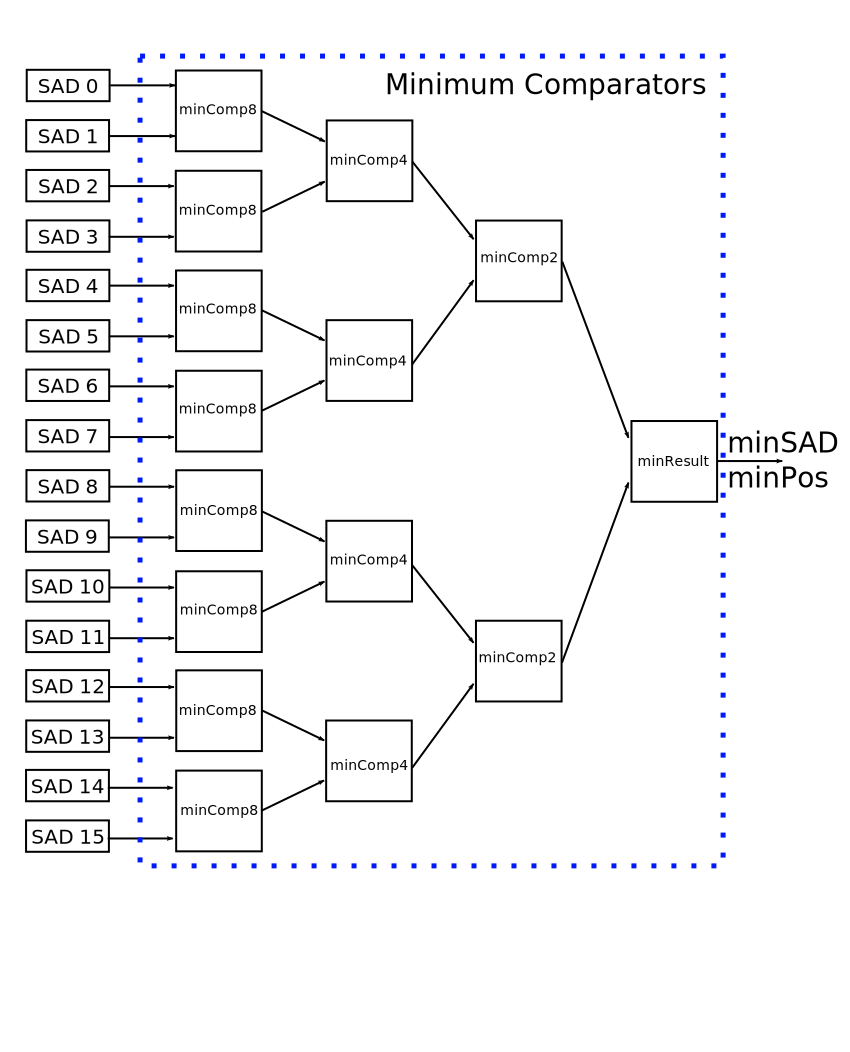
\includegraphics[width=150mm]{figures/minComparator.png}
		\captionfonts
		\caption{The minimum comparator tree designed to quickly find the minimum value and corresponding index out of the 16 SAD values that are calculated for one pixel.}
		\label{fig:minComp}
	\end{center}
\end{figure}


\subsection{SAD Wrapper}

\begin{figure}[h]
	\begin{center}
		\includegraphics[width=100mm]{figures/sad_wrapper_rtl.png}
		\captionfonts
		\caption{The SAD wrapper that encompasses the SAD algorithm and minimum comparator. It interacts with the top level.}
		\label{fig:sadWrapper_rtl}
	\end{center}
\end{figure}


\subsection{Top Level}

\begin{figure}[h]
	\begin{center}
		\includegraphics[width=150mm]{figures/top_level_rtl.png}
		\captionfonts
		\caption{The overview of the structure used for implementing the 9x9 window. The 7x7 window has two less SAD and minComp each.}
		\label{fig:topLevel_rtl}
	\end{center}
\end{figure}

\section{FPGA and Computer Communication}



\subsection{FPGALink}





\chapter{Experiments and Results}
Experiments and Results


\chapter{Conclusions}
\label{sec:concl}

For image processing, the more operations that can be parallelized, the faster images can be processed. However, as parallelism is increased, the amount of hardware required also is increased. It could be possible to parallelize a SAD algorithm, or most image processing methods, to only take a few clock cycles to process the whole image (i.e. every SAD calculation for an image pair happening simultaneously). Unfortunately, the area required on an FPGA would be a lot more than what was implemented in this paper. The cost of an FPGA that could handle that amount of hardware would be very cost prohibitive and not something a club or hobbyist could readily use for a robotics project. There does come a point at which the frames per second of disparity maps produced exceeds the speed that the other parts of the robot can process, which is unnecessary cost. So the FPGA board only needs to be able to handle a SAD implementation up to a certain frame rate, which depends on the requirements of the application for the robot.

The smaller the image size, the higher the frame rate, as shown in Figure~\ref{fig:frameRate}. Once the number of pixels in an image goes below 180,000 for the 7x7 window implementation or 140,000 for the 9x9 window implementation, the frame rate approaches 30 frames per second, which is good for humans. For robots, a frame rate of 10 should be sufficient for most tasks that do not require a higher frame rate. Both the 9x9 and 7x7 window implementations were shown be above 10 frames per second for an image size of 640x480.

\begin{figure}
	\begin{center}
		\includegraphics[width=100mm]{figures/frameRate.png}
		\captionfonts
		\caption{Frame rate comparison of different image sizes.}
		\label{fig:frameRate}
	\end{center}
\end{figure}

Between the 9x9 window implementation and the 7x7 window implementation, unless a higher frame rate is needed, the 9x9 is better than the 7x7. While 7x7 has a higher frame rate, 9x9 produces a better quality disparity map with less noise and requires fewer hardware resources.

This modular implementation of the SAD algorithm has the potential to be used for FPGA implementations in autonomous mobile robotic applications.

\chapter{Future Work}

The next steps are to get a fully functional stereo vision implementation on the Atlys board that uses the SAD module presented in this paper. The Atlys board has a 1 GB DDR RAM chip, which could be used to buffer the images from the VmodCAM stereo camera module~\cite{atlysBoard}. The left and right images from the VmodCam could be buffered to the DDR RAM and then sections of the buffered images could be sent to the SAD module to obtain the disparity values. With the correct timing and buffering, both or one of the images and the disparity image could then be sent off board to a computer on a robot to use the image and depth data to navigate and interact with the world.

After a fully functional implementation on the Atlys board is working, a custom FPGA board could be designed and manufactured. The custom board only needs the functionalities of the Atlys board in order to: communicate with the computer, obtain images from the stereo cameras, buffer the images on the DDR RAM, and process everything else on the FPGA IC. A custom board without the extra peripherals on board has the potential to further reduce the cost of a stereo vision FPGA board. Also, the stereo cameras could be built into the board to reduce the cost of hardware needed for connections.

Furthermore, replacing the FPGA IC used on the Atlys board with one that has a clock frequency higher than 100 MHz or more space while keeping the cost of the IC around the same as the Atlys board FPGA IC is way to speed up the SAD calculation time and increase the frame rate.

When all is said and done, having robots readily able to have better and less expensive "eyes" to perceive the world around them in greater depth will be pretty neat.

% ------------- End main chapters ----------------------

\clearpage
\bibliographystyle{plain}
\bibliography{references}

\begin{appendix}
\addcontentsline{toc}{chapter}{\appendixnamelower}
\chapter{Absolute Difference 9x9 Window Code Snippet}
\label{sec:appdxA}

\definecolor{mygreen}{rgb}{0,0.6,0}

\lstset{
	language=VHDL,
	basicstyle=\footnotesize,
	commentstyle=\color{mygreen},
	keywordstyle=\color{blue}, 
	tabsize=3
}

\begin{lstlisting}

-- Assign greater value to more and smaller to less
IF (search_window(ndx) < template_window(ndx)) THEN 
	more <= template_window(ndx);
	less <= search_window(ndx);
ELSE
	less <= template_window(ndx);
	more <= search_window(ndx);
END IF;

-- Subtraction IP CORE, sub = more - less
subber : subtr_core
	PORT MAP (
		a => more,
		b => less,
		s => sub
	);
	
\end{lstlisting}
\chapter{Absolute Difference 7x7 Window Code Snippet}
\label{sec:appdxB}

\definecolor{mygreen}{rgb}{0,0.6,0}

\lstset{
	language=VHDL,
	basicstyle=\footnotesize,
	commentstyle=\color{mygreen},
	keywordstyle=\color{blue}, 
	tabsize=3
}

\begin{lstlisting}

-- Assign greater value to more and smaller to less
-- Loop is unrolled in hardware, 7 assignments occur simultaneously
FOR i IN 0 TO 6 LOOP
	IF (search_window(ndx+(7*i)) < template_window(ndx+(7*i))) THEN 
		more(i) <= template_window(ndx + (7*i));
		less(i) <= search_window(ndx + (7*i));
	ELSE
		less(i) <= template_window(ndx + (7*i));
		more(i) <= search_window(ndx + (7*i));
	END IF;
END LOOP;

-- Subtraction IP CORE, sub(i) = more(i) - less(i)
g_differ_10 : FOR i IN 0 TO 6 GENERATE
	i_subber : adder_10
		PORT MAP (
			a => more(i),
			b => less(i),
			s => sub(i)
		);
END GENERATE g_differ_10;

\end{lstlisting}
\chapter{Minimum Comparator Code}
\label{sec:appdxC}

\definecolor{mygreen}{rgb}{0,0.6,0}

\lstset{
	language=VHDL,
	basicstyle=\footnotesize,
	commentstyle=\color{mygreen},
	keywordstyle=\color{blue}, 
	tabsize=3
}

\begin{lstlisting}

-- Constantly assign inputs
sad0 <= sad0_I;
pos0 <= pos0_I;
sad1 <= sad1_I;
pos1 <= pos1_I;

-- Comparison
PROCESS(clk_I)
begin
	IF (RISING_EDGE(clk_I)) THEN
		IF (sad1 < sad0) THEN
			sad_out <= sad1;
			pos_out <= pos1;
		ELSE
			sad_out <= sad0;
			pos_out <= pos0;
		END IF;
	END IF;
END PROCESS;

-- Constantly assign outputs
sad_O <= sad_out;
pos_O <= pos_out;

\end{lstlisting}
\chapter{Testbench Simulations}
\label{sec:appdxD}

\begin{sidewaysfigure}
	\begin{center}
		\includegraphics[height=8cm]{figures/buffer_testbench_9x9_4.png}%testbench_simulation_9x9.png}
		\captionfonts
		\caption{Testbench simulation for the 9x9 window implementation.}
		\label{fig:tb_9x9}
	\end{center}
\end{sidewaysfigure}


\begin{sidewaysfigure}
	\begin{center}
		\includegraphics[height=8cm]{figures/buffer_testbench_7x7_2.png}
		\captionfonts
		\caption{Testbench simulation for the 7x7 window implementation.}
		\label{fig:tb_7x7}
	\end{center}
\end{sidewaysfigure}

\chapter{Python3 Serial SAD Algorithm}
\label{sec:appdxE}

\definecolor{mygreen}{rgb}{0,0.6,0}

\lstset{
	language=Python,
	basicstyle=\footnotesize,
	commentstyle=\color{mygreen},
	keywordstyle=\color{blue}, 
	tabsize=4
}

\begin{lstlisting}
# Parameters for 9x9 window size SAD Algorithm
winSize = 9
dispRange = 16
dispRow = 4
win = (int)(winSize/2)
ncol = (dispRow-1) + dispRange + (winSize-1)
dispH = height - (winSize-1)
dispW = width - (ncol - dispRow)

# Serial SAD Algorithm
for row in range(dispH):
	sadArray = numpy.zeros((dispW, dispRange), dtype = 'i')
	for i in range(dispW):
		for j in range(dispRange):
			for m in range(-win, (win+1)):
				for n in range(-win, (win+1)):
					sadArray[i][j] += \
						abs(templateBuff[row+m+win][n+i+win] - \ 
						searchBuff[row+m+win][n+i+j+win])
	disparityArray = sadArray.argmin(axis=1)
	disparityAll[row] = disparityArray
\end{lstlisting}

The full code for the Python3 SAD Algorithm can be found on github:
\\\path{https://github.com/cccitron/mastersThesis/tree/master/pythonSAD}

%\include{AppendixF}
\end{appendix}

\end{document}